\documentclass{standalone}
\usepackage{tikz}
\usetikzlibrary{positioning}

\begin{document}
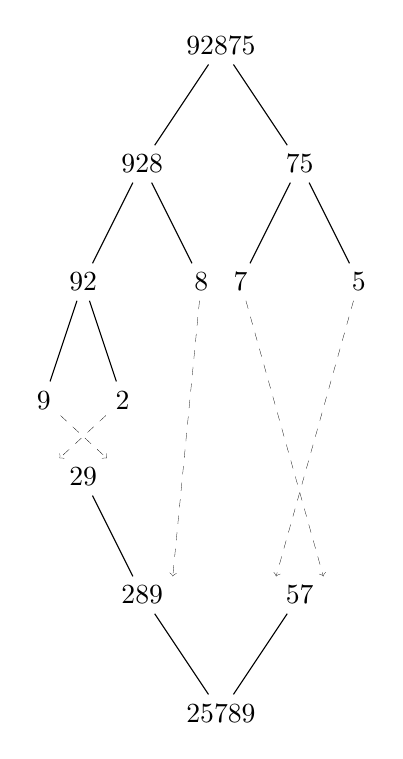
\begin{tikzpicture}[
    level 1/.style={sibling distance=20mm},
    level 2/.style={sibling distance=15mm},
    level 3/.style={sibling distance=10mm}
]
    \node(start){92875}
        child {node {928}
            child {node {92}
                child {node (a) {9}}
                child {node (b) {2}}
                }
            child {node (c) {8}}
            }
        child {node {75}
            child {node (d) {7}}
            child {node (e) {5}}
            };

    \node[below = 8cm of start] (ziel) {25789} [grow'=up]
        child {node (B) {289}
            child {node (A) {29}}
            child[white]
            }
        child {node (C) {57}};

    \draw[ultra thin, dashed, ->] (b) -- (A.north west); 
    \draw[ultra thin, dashed, ->] (a) -- (A.north east);
    \draw[ultra thin, dashed, ->] (c) -- (B.north east);
    \draw[ultra thin, dashed, ->] (d) -- (C.north east);
    \draw[ultra thin, dashed, ->] (e) -- (C.north west);
\end{tikzpicture}
\end{document}